\documentclass[a4paper,11pt,latin]{moderncv}
\usepackage[utf8]{inputenc}
\usepackage[T1]{fontenc}
\usepackage[ngerman]{babel}
\usepackage{amsmath}
\moderncvstyle{classic}
\moderncvcolor{blue}
\usepackage{pdfpages}
\usepackage{graphicx}
\usepackage{currvita}
\usepackage{pdfpages}

%\def\Stelle{IT-Kundenbetreuer}
\def\Firma{Gff Finanz- und Personalwirtschaftssysteme GmbH}
\def\Ansprechpartner{Josef Luhmer}
\def\Strasse{Rennweg 60}
\def\PLZ{56626 Andernach}

\firstname{Sascha}
\familyname{Manns}
\address{Maifeldstrasse 10}{56727 Mayen}
\phone{+49-2651-40~14~045}
\email{Sascha.Manns@bdvb.de}
\homepage{http://saigkill.github.io}

\photo[20mm][0mm]{./Sascha1p.jpg}

\title{Curriculum Vitae}
\quote{"Mehr als die Vergangenheit interessiert mich die Zukunft, denn in ihr gedenke ich zu leben", Albert Einstein}

\begin{document}
% Anschreiben und Deckblatt
%\includepdf{../Anschreiben/bwanschreiben} %bei Bedarf uncommenten
%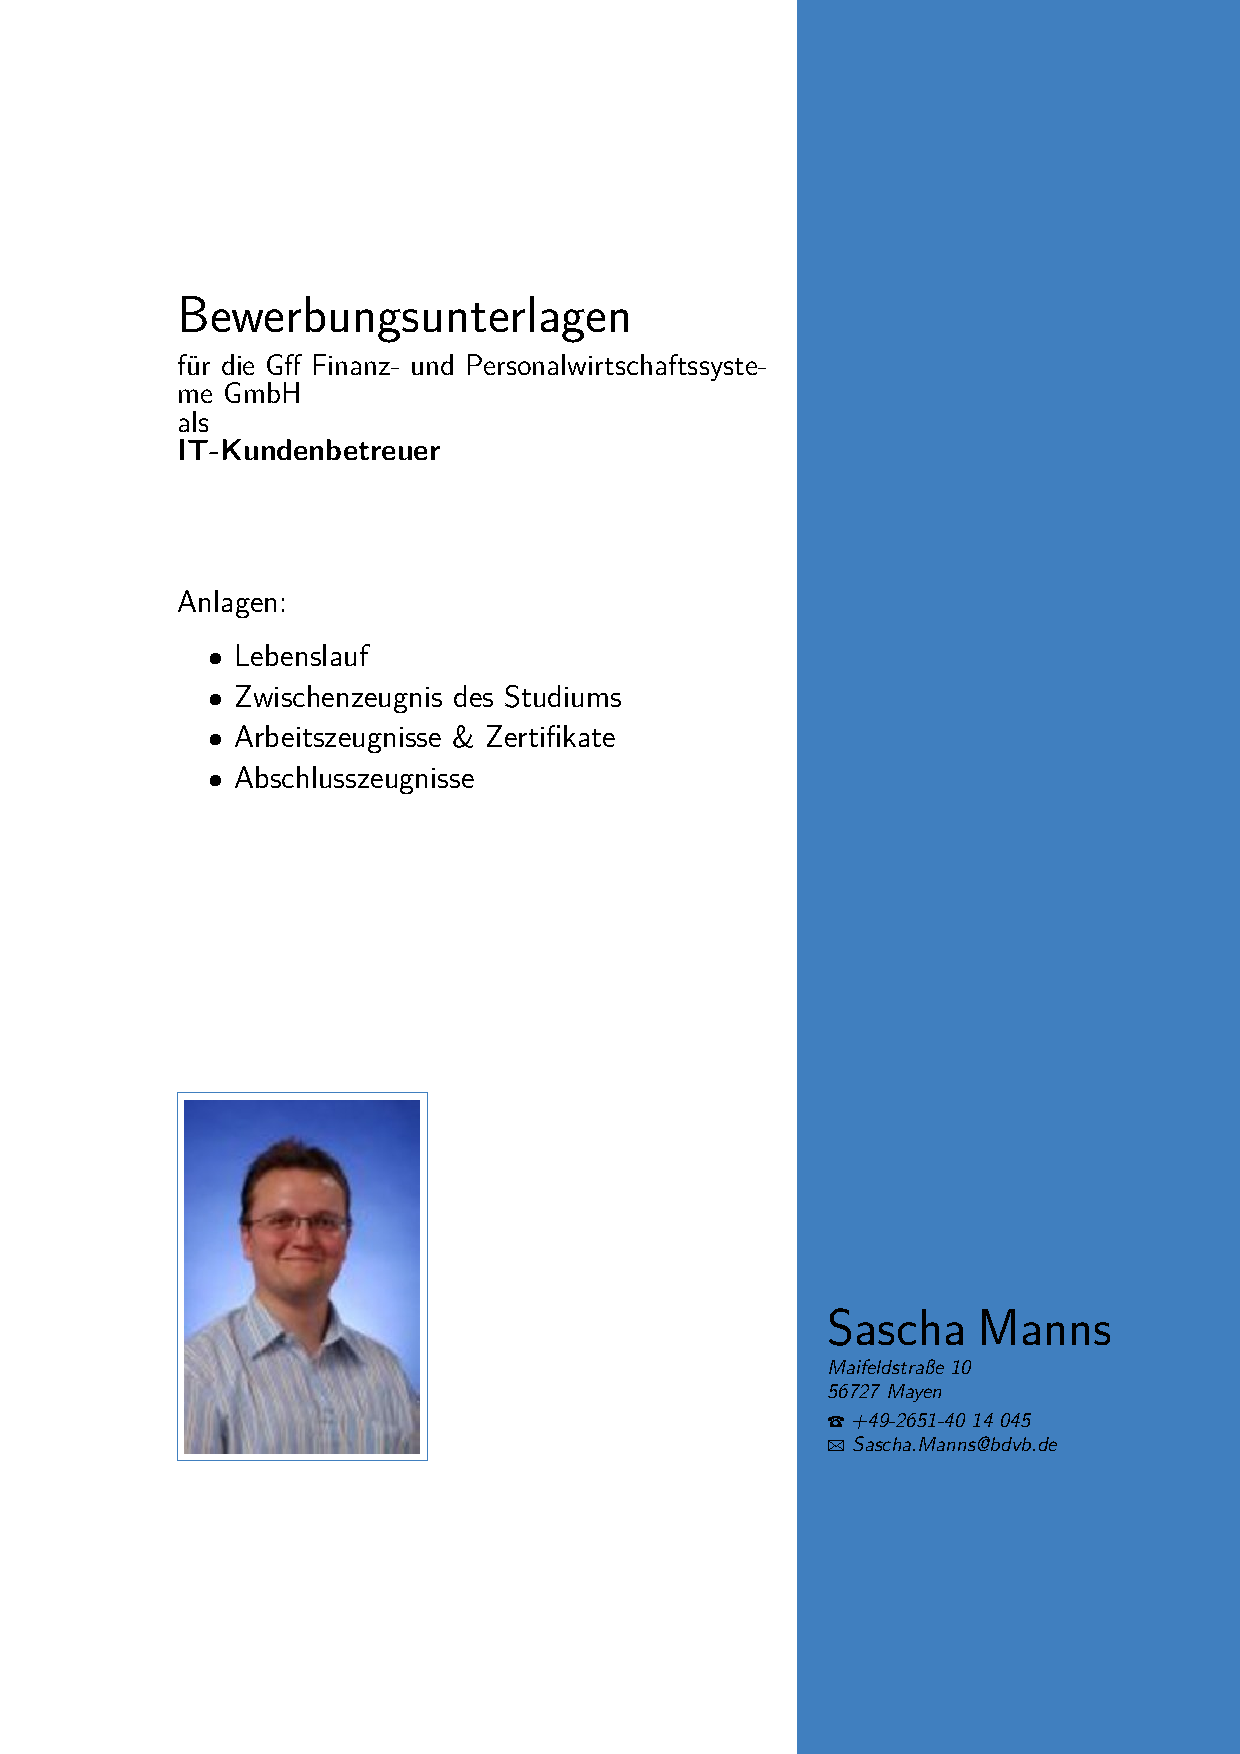
\includepdf{../Deckblatt/Deckblatt}

\makecvtitle
\section{Berufsleben}
\cventry{02/2014--jetzt}{IT-Supporter (Dispatcher)}{ITSCare}{Neuwied}{}{}
\cventry{07/2012--06/2012}{Community \& Support Ag./Buchautor/Screencsats}{open-slx~GmbH}{Nürnberg}{}{}
\cventry{07/2011--07/2012}{Langzeitpraktikum}{open-slx~GmbH}{Nürnberg}{}{}
\cventry{07/2010--07/2011}{Freiwillige Mitarbeit}{open-slx~GmbH}{Nürnberg}{}{}
\cventry{06/2007--07/2010}{Kurzzeitiger Aussetzer aufgrund gesundheitlicher Probleme (Tod des Vaters)}{ehrenamtl. Tätigkeiten.}{}{}{}
\cventry{08/2000--06/2007}{Ersatzdienst (zum Zivildienst)}{WTG}{Selters}{}{}
\cventry{08/1998--08/2000}{Kaufmann im Einzelhandel}{Auto Deschner GmbH}{Mendig}{}{}
\section{Weiterbildung \& Zertifikate}
\cventry{10/2013--jetzt}{Web Engeneering I: Grundlagen der Webentwicklung}{TH Mittelhessen}{MOOC}{}{}
\cventry{06/2013}{BDVB Kompetenzpass für Ökonomen}{BV Deutscher Volks- und Betriebswirte}{Düsseldorf}{}{}
\cventry{04/2013--jetzt}{Studium zum staatl. gepr. Betriebswirt Schwerpunkt Wirtschaftsinformatik}{ILS Fernschule}{Hamburg}{}{}
\cventry{04/2013}{Schlüsselkompetenzen Kompakt}{DIS AG}{}{}{}
\section{Ausbildung}
\cventry{08/1995--08/1998}{Ausbildung zum Kaufmann im Einzelhandel}{Auto Deschner GmbH}{Mendig}{}{}
\section{Ehrenamtliche Tätigkeiten}
\cvitemwithcomment{2013--jetzt}{mUXCamp 2014 Organisationsteam}{Planung des nächsten Camps}{}
\cvitemwithcomment{2013--jetzt}{BV Deutscher Volks- und Betriebswirte}{FG Wirtschaftsinformatik}{}
\cvitemwithcomment{2013--jetzt}{Gesellschaft für Informatik}{FB Wirtschaftsinformatik \& FB Informatik und Gesellschaft}{}
\cvitemwithcomment{2013--jetzt}{Forum Informatiker für Frieden und \\gesellschaftliche Verantwortung}{}{}
\cvitemwithcomment{2008--jetzt}{openSUSE Linux Projekt}{RPM-Packaging}
\section{Computerkenntnisse}
\cvdoubleitem{OS:}{Linux, Windows 3.11 - XP}{Office:}{Alle üblichen}
\cvdoubleitem{Programmier\\-sprachen:}{Shell (Bash), Ruby}{Administration:}{Linux/Unix}
\cvitem{Packaging:}{RPM (Compiling, Testing)}
\cvitem{Translations:}{FreeMedForms, KVirustotal (Übersetzung EN $\triangleright$ DE)}
\cvitem{Textsatz:}{\LaTeX, DocBook4.5, XSL-FO}
\cvitem{Multimedia:}{Pod \& Screencastproduktion}
\cvitem{Produkt\\gestaltung:}{Handbucherstellung, Supportdatenbank, Webpräsentation}
\cvitem{Webservices:}{Apache2, Joomla, Owncloud, Wordpress, Mediawiki, Cloudcontrol Appliances}
\cvitem{Wissens\\management:}{Geschftl. Wiki, Geschftl. Soziale Netzwerke}
\cvitem{Erweiterte Kenntnisse in:}{Warenwirtschaftssysteme, Auftragsmanagementsysteme, OTRS, Mantis, Amsys, IDM}
\section{Sprachkenntnisse}
\cvitem{Deutsch}{Muttersprache}
\cvitem{Englisch}{gut} 
\section{Hard Skills}
\cvlistitem{Erfahrungen mit Gründung internationaler (IT-Projekt)-Teams \& Koordination in bis zu 13 Sprachen}
\cvlistitem{Erfahrungen im Umgang mit Menschen aus anderen Kulturkreisen}
\cvlistitem{Fachvorträge}
\cvlistitem{Erfahrungen in Öffentlichkeitsarbeit \& Social Media Management (für IT-Produkte)}
\section{Publikationen}
\cvlistitem{Sascha Manns et al.: \textit{openSUSE Weekly News} \\2009-2012 Web,URL: \url{http://tinyurl.com/mmkpnyj}}
\cvlistitem{Sascha Manns et al.: \textit{open-slx Wochenrückblick} \\2013 Web, ISSN:2195-5344, URL: \url{http://tinyurl.com/l2zow4v}}
\cvlistitem{Sascha Manns: \textit{Praxis Dr. Datenbrief - Ein Selbstversuch} \\2010 Berlin, Die Datenschleuder 94 Seite 37, ISSN: 0930-1054, URL: \url{http://ds.ccc.de/pdfs/ds094.pdf}}
\cvlistitem{Sascha Manns/Jens Köke: \textit{Startup Guide für Balsam Professional} 2011 Nürnberg, Boxprodukt, D-NB-URL: \url{http://d-nb.info/1016808844}}
\cvlistitem{Sascha Manns: \textit{Plasma Active Handbook} 2013 Lulu Press Inc. \\Web: \url{http://pactivehandbook.sourceforge.net}, \\ISBN: 978-1-291-57787-7 (englisch) und ISBN: 978-1-291-57705-1 (deutsch), D-NB-URL: \url{http://d-nb.info/1042698783}}
\section{Social Media Profile}
\cvitem{Google+}{\url{https://plus.google.com/113047759144486797915}}
\cvitem{Facebook}{\url{http://www.facebook.com/sascha.manns}}
\cvitem{Xing}{\url{https://www.xing.com/profile/Sascha\_Manns2}}
\cvitem{Linked.in}{\url{http://de.linkedin.com/in/saigkill/}}
\section{Interessen}
\cvlistdoubleitem{Literatur (IT/Wirtschaft/Philosphie)}{Bücher verfassen}
\cvlistdoubleitem{Wandern}{Netzwerken (Real Life)}

%\vspace{1.0cm}

%\begin{center}
%
\includegraphics[scale=0.7]{spool/signatur.png} \\
%\begin{tabular}{@{}l@{}}
%\\ $\frac{}{\strut\textnormal{Sascha Manns, Mayen den \today}}$
%\end{tabular}
%\end{center}

%\section{Anhang}
%---------------------------------------------------------------------------
% Include PDF

\includepdf{spool/thm-webeng1}

\includepdf{spool/zwzils}
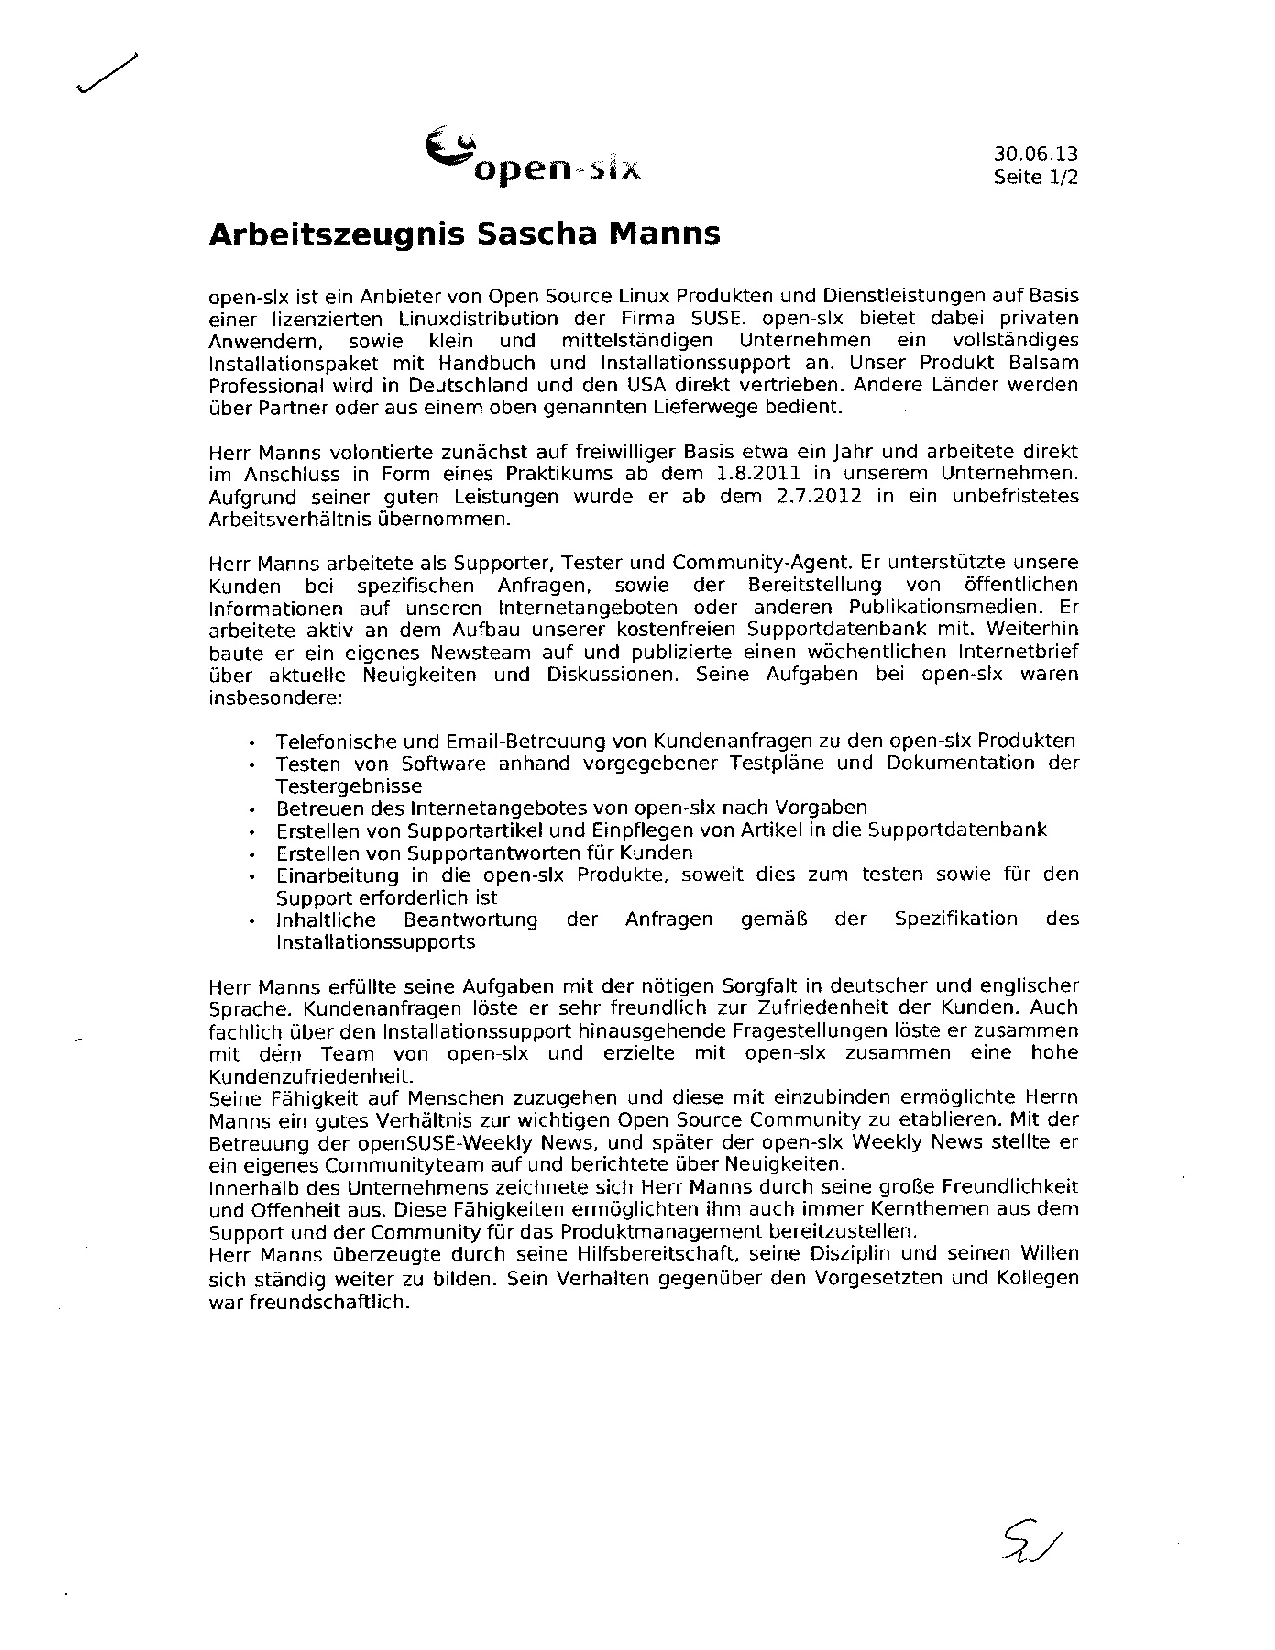
\includepdf{spool/openslx}

\includepdf{spool/openslx1}

\includepdf{spool/kompetenzpass12013}

\includepdf{spool/Zertifikat_Sascha_Manns1}

\includepdf{spool/wtg}

\includepdf{spool/ihk}


\end{document}
